\chapter{Subsystem: Operator Control and User Interface}

\section{User-Interface Design} The existing user interface uses a large black-box with a joystick, a series of buttons and switches, and a small LED display.  The box provides all major functionality that an operator could need to interface with the vehicle.  An operator can throttle, break, steer, change gears and force the vehicle to an emergency stop all from the box.  This box; however, is not the best solution for our design.

Our design requires displaying a large amount of data to an operator.  The small LED display on the box will not work for this goal.  The black-box is also not desirable because it is hard to extend.  There are a finite number of button and switches, many of which have already been programmed for essential functionality.  Our design needs a user-interface that is:
\begin{itemize}
	\item easy to use
    \item can handle displaying large amounts of information to the operator but does not overwhelm them with the info
    \item can be extended to provide extra functionality in the future \ldots
\end{itemize}
  
Given these requirements, we have decided to implement a web-based user-interface.  Operators will interact with the vehicle through a web-page.  This web-page will display the incoming information from the sensor packages on the vehicle and incoming information about the state of the vehicle itself.  Most operators should be familiar with how to navigate a web-page from interacting with them on a regular basis on their own, so the interface should feel intuitive and natural to most operators.  There is also a vast amount of research on how to develop friendly and easy-to-use web-pages that our team can leverage when implementing our web-based user-interface.

\section{RobotWebTools and the ROS Control Center}Initially our team thought about replacing the black-box entirely and allow user's to drive the vehicle by using a gamepad controller.  Google Chrome and Mozilla Firefox both natively support gamepad interactions via the Gamepad API; however, we abandonned this goal to focus more on visualizing the incoming sensor data.  The black-box already contains the functionality for driving the vehicle and the Gamepad API is still in active development and is not at a state where we would feel comfortable using it for driving a vehicle.

After a large amount of research on how to visualize ROS data via a web-page we discovered the RobotWebTools group \cite{robotwebtools}. This group was actively developing tools for connecting to ROS from a website.  The architecture works by running a webserver with ROS, and then having HTML pages connect to that webserver via Javascript.  The Javascript library is meant to replicate the ROS architecture.  It subscribes to nodes, and when that node publishes an event, the webserver captures it, converts it into a JSON object, and then sends that object to the Javascript library.  The Javascript library is then free to work with that data.

The RobotWebTools provide the low end infrastructure for building a web-based user-interface with ROS.  We started to design our user-interface to be a single page view of the state of the vehicle and visualize all of the sensor data.  We decided on this because a user needs to be able to focus on driving the vehicle, and forcing them to have to click through tabs to find the data that they needed seemed unreasonable.  The sheer amount of data that we are processing makes this difficult.  We have a handful of sensors and cameras, the LIDAR, and vehicle state and location data to display in one page.  Furthermore, we need our interface to be flexible and dynamic so that it can subscribe to all of the necessary nodes immediately without needing to be reconfigured.  If we add new nodes for new sensors on the vehicle, then we want our user-interface to be able to identify and display that data with little effort.

While researching how to accomplish our user-interface, we discovered that someone else had recently publicly posted a web-based user-interface that was built on top of the RobotWebTools libraries.  The project is called the ROS Control Center and is an AngluarJS project which provides a template for how to build a web-based user-interface to visualize ROS data \cite{roscontrolcenter}.

\begin{figure}[H]
\centerline{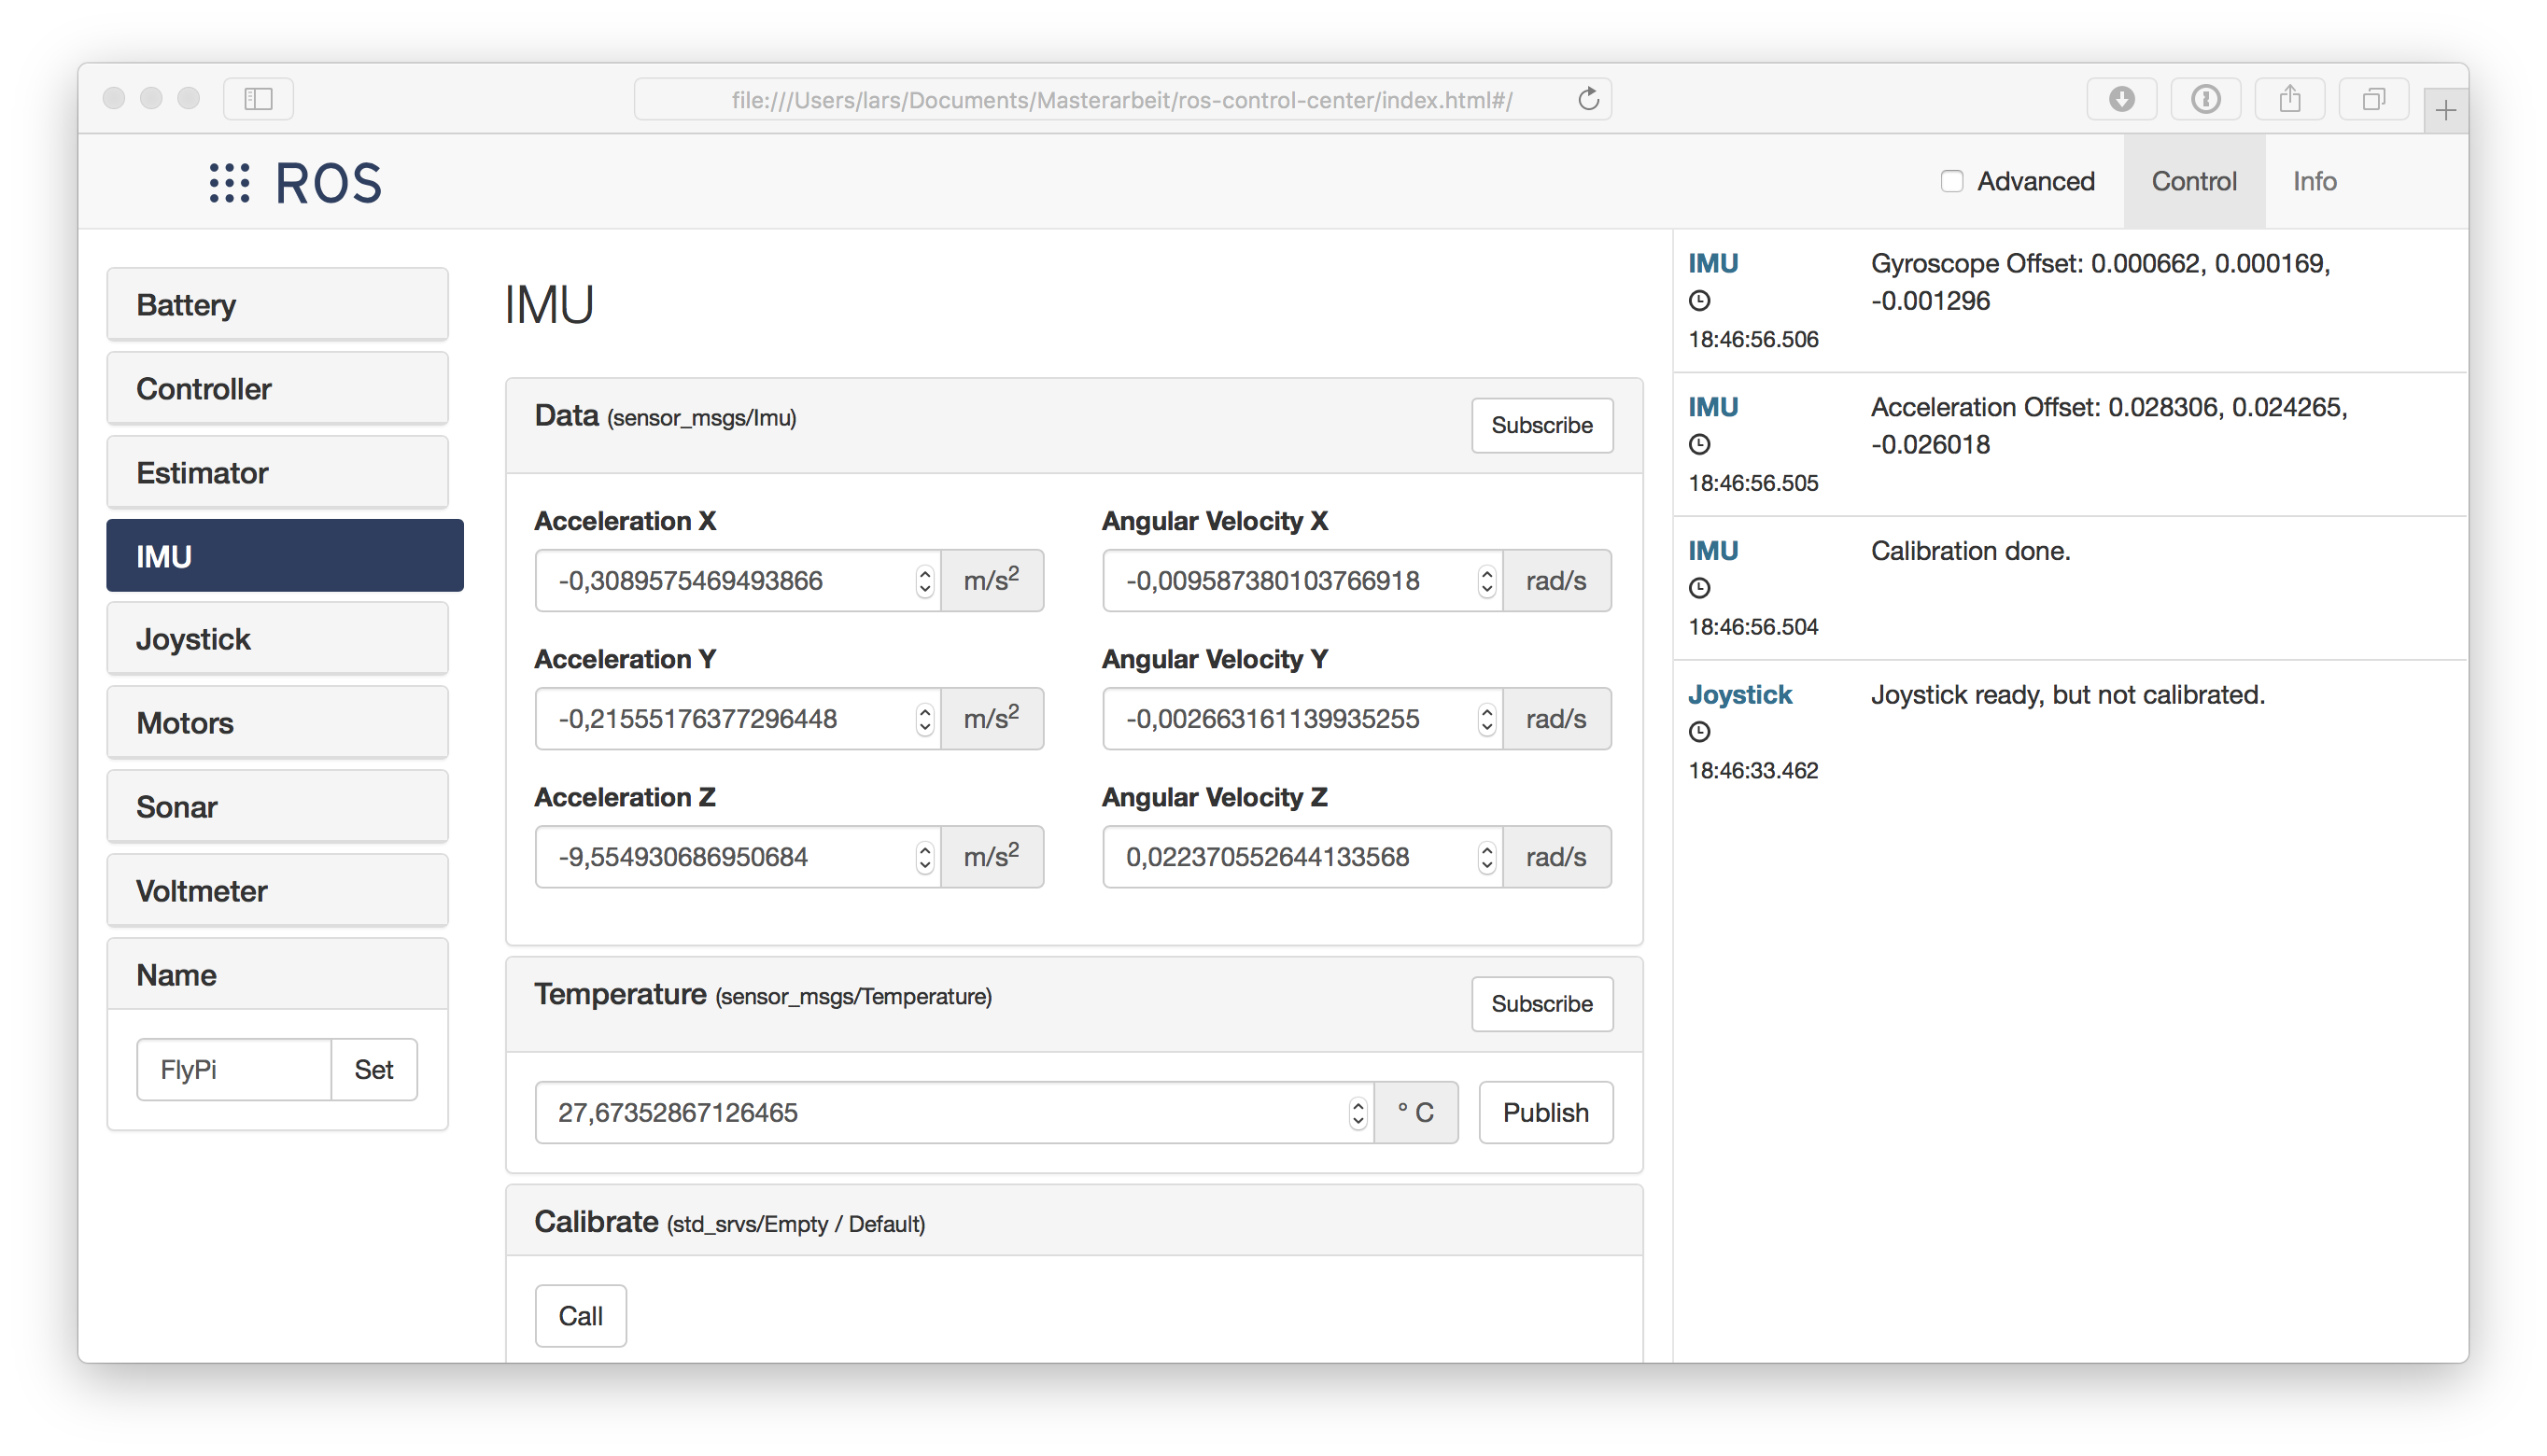
\includegraphics[angle=0,width=1\linewidth]{ros_control_center_screenshot}}
\caption[]{ROS Control Center}
\label{fig:roscontrolcenter}
\end{figure}

As seen in \ref{fig:roscontrolcenter}, the ROS Control center comes prepackaged with visualization for a variety of default ROS packages.  The ROS Control Center provides the flexibility and dynamism that we are looking for.  The ROS Control Center works by asking the RobotWebTools webserver for all nodes that are currently publishing messages.  These nodes and messages have to have a unique name as part of the ROS architecture.  The ROS Control Center leverages this feature.  Each node has a directory, and each message has an HTML file with the code needed to visualize that message.  When the ROS Control Center recognizes a node, it adds the node to the left-side navigation bar.  Then, the ROS Control Center embeds the HTML code for visualizing the indivdual messages into the page.  This way, a user can click on a particular node's name, and then see all of data for all of the messages that belong to that node.  Writing these HTML files for each message is fairly simple to do because the ROS Control Center handles all of the data processing.

The ROS Control Center is not a perfect solution.  It does not provide a one page view of the vehicle.  It also does not have any standard way for providing graphs.  It displays all data as a single value that live updates as it receives more information.  This works for features like cameras, but for our enviromental sensors, its helpful to be able to view the sensor data over a period of time, and not just see the most recent value.  The ROS Control Center also does not provide any way to handle the idea of thresholds and warnings. Many of the enviromental hazards we are trying to detect have safe and unsafe thresholds.  We want our user-interface to be able to provide feedback to the user when the unsafe thresholds are exceeded to quickly alert the user that there is a problem.

These are all features that can be added to the ROS Control Center.  Since each message is given it's own HTML page, we can write the Javascript logic in those pages to handle alerts for safe and unsafe conditions and build livestream plots in those pages too.  We can also build a page that uses the data from multiple messages and displays them in one page.  Adding these features on top of the ROS Control Center will meet our design requirements and goals.

\section{Network for Internet Communication}The RobotWebTools libraries and the ROS Controller Center assume that there is an internet connection between ROS and the device running the ROS Controller Center.  We plan on deploying our vehicle in rugged, off-road terrain where an existing internet connection is not necessarily available.  To deal with this problem, we purchased a high-power router that sits on the vehicle.  On the vehicle we run the RobotWebTools rosbridge\char`_server package and a small HTTP web-server.  The rosbridge\char`_server package handles translating ROS messages to a JSON format so that the web-client can use the data.  The HTTP Server on the vehicle handles serving the web-client with the HTML and Javascript files that are necessary to run the ROS Control Center.

\begin{figure}[H]
\centerline{\includegraphics[angle=0,width=1\linewidth]{NetworkRover}}
\caption[]{Network architecture to enable the user-interface}
\label{fig:NetworkRover}
\end{figure}

By placing the HTTP server on the vehicle, we allow any device on the network provided by our router to connect to our edited ROS Control Center.  We could have multiple devices and users connected and viewing the data.  It also means that there is no setup that has to be done on the device other than connecting to the network.  The network is password protected so only the people who need access will be able to interface with the vehicle.  